\documentclass{assignment-373}
\usepackage{mathabx}
\usepackage{tikz}


\anum{2}
\course{CSC373}
\duedate{Oct 3, 2020}
\filename{ps2.pdf, ps2.tex}

\begin{document}

\think

\textbf{Please see the course information sheet for the late submission
  policy.}

\textbf{[15 points]}

  Sushant has played a lot of Tic-Tac-Toe in his early years, and his
  favorite mark was $\bigtimes$. So whenever he sees a grid, he's
  looking to find the biggest $\bigtimes$ symbol he can fit in it.

  You are given an $n \times n$ array with entries in 0 or 1. 0
  indicates that that location is empty, and 1 indicates that the
  location is filled. Your goal is to determine the largest size of an
  $\bigtimes$ symbol that can be filled in the grid while utilizing
  only the 0 locations. The following figures below demonstrate
  $\bigtimes $ with sizes 1, 2, and 3 respectively (a zero sized
  $\bigtimes$ would have no blue squares).
  
  \begin{minipage}{0.2\textwidth}
    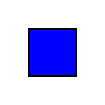
\begin{tikzpicture}
      [%%%%%%%%%%%%%%%%%%%%%%%%%%%%%%
      box/.style={rectangle,draw=black,thick, minimum size=0.6cm},
      ]%%%%%%%%%%%%%%%%%%%%%%%%%%%%%%
      
      \node[box,fill=blue ] at (0.6*0,0.6*0){};  
    \end{tikzpicture}
  \end{minipage}
  \begin{minipage}{0.3\textwidth}
    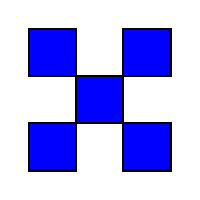
\begin{tikzpicture}
      [%%%%%%%%%%%%%%%%%%%%%%%%%%%%%%
      box/.style={rectangle,draw=black,thick, minimum size=0.6cm},
      ]%%%%%%%%%%%%%%%%%%%%%%%%%%%%%%
      
      \node[box,fill=blue ] at (0.6*0,0.6*0){};  
      \node[box,fill=blue ] at (0.6*1,0.6*1){};  
      \node[box,fill=blue ] at (0.6*2,0.6*2){};  
      \node[box,fill=blue ] at (0.6*0,0.6*2){};  
      \node[box,fill=blue ] at (0.6*2,0.6*0){};  
    \end{tikzpicture}
  \end{minipage}
  \begin{minipage}{0.4\textwidth}
    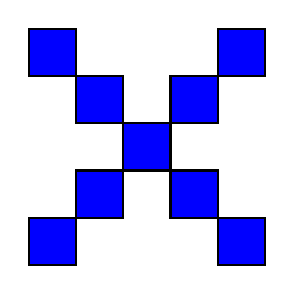
\begin{tikzpicture}
      [%%%%%%%%%%%%%%%%%%%%%%%%%%%%%%
      box/.style={rectangle,draw=black,thick, minimum size=0.6cm},
      ]%%%%%%%%%%%%%%%%%%%%%%%%%%%%%%
      
      \node[box,fill=blue ] at (0.6*0,0.6*0){};  
      \node[box,fill=blue ] at (0.6*1,0.6*1){};  
      \node[box,fill=blue ] at (0.6*2,0.6*2){};  
      \node[box,fill=blue ] at (0.6*3,0.6*3){};  
      \node[box,fill=blue ] at (0.6*4,0.6*4){};  
      \node[box,fill=blue ] at (0.6*0,0.6*4){};  
      \node[box,fill=blue ] at (0.6*1,0.6*3){};  
      \node[box,fill=blue ] at (0.6*3,0.6*1){};  
      \node[box,fill=blue ] at (0.6*4,0.6*0){};  
    \end{tikzpicture}
  \end{minipage}
  
  In the example grids drawn below, the squares with 1 in the input
  array are filled with black color, and all the squares colored blue
  or white are 0 locations. The blue squares visualize an $\bigtimes$
  with the biggest possible size that can be fit inside the grid using
  only non-black locations.

  \begin{minipage}{0.4\textwidth}
    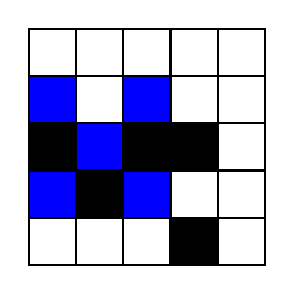
\begin{tikzpicture}
      [%%%%%%%%%%%%%%%%%%%%%%%%%%%%%%
      box/.style={rectangle,draw=black,thick, minimum size=0.6cm},
      ]%%%%%%%%%%%%%%%%%%%%%%%%%%%%%%
      
      \foreach \x in {0,1,...,4}{
        \foreach \y in {0,1,...,4}
        \node[box] at (\x*0.6,\y*0.6){};
      }
      
      \node[box,fill=black ] at (0.6*1,0.6*1){};  
      \node[box,fill=black ] at (0.6*0,0.6*2){};  
      \node[box,fill=black ] at (0.6*3,0.6*0){};  
      \node[box,fill=black ] at (0.6*3,0.6*2){};  
      \node[box,fill=black ] at (0.6*2,0.6*2){};  
      
      \node[box,fill=blue ] at (0.6*0,0.6*1){};  
      \node[box,fill=blue ] at (0.6*1,0.6*2){};  
      \node[box,fill=blue ] at (0.6*2,0.6*3){};  
      \node[box,fill=blue ] at (0.6*0,0.6*3){};  
      \node[box,fill=blue ] at (0.6*2,0.6*1){};  
    \end{tikzpicture}
  \end{minipage}
  \begin{minipage}{0.6\textwidth}
    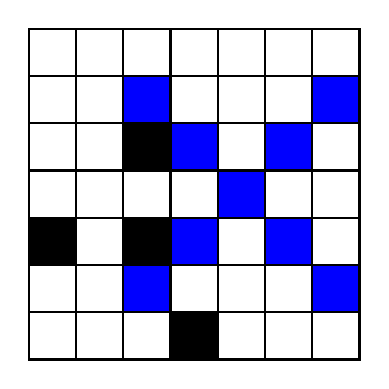
\begin{tikzpicture}
      [%%%%%%%%%%%%%%%%%%%%%%%%%%%%%%
      box/.style={rectangle,draw=black,thick, minimum size=0.6cm},
      ]%%%%%%%%%%%%%%%%%%%%%%%%%%%%%%
      
      \foreach \x in {0,1,...,6}{
        \foreach \y in {0,1,...,6}
        \node[box] at (\x*0.6,\y*0.6){};
      }
      
      \node[box,fill=black ] at (0.6*2,0.6*4){};  
      \node[box,fill=black ] at (0.6*0,0.6*2){};  
      \node[box,fill=black ] at (0.6*3,0.6*0){};  
      \node[box,fill=black ] at (0.6*3,0.6*2){};  
      \node[box,fill=black ] at (0.6*2,0.6*2){};  
      
      \node[box,fill=blue ] at (0.6*2,0.6*1){};  
      \node[box,fill=blue ] at (0.6*3,0.6*2){};  
      \node[box,fill=blue ] at (0.6*4,0.6*3){};  
      \node[box,fill=blue ] at (0.6*5,0.6*4){};  
      \node[box,fill=blue ] at (0.6*6,0.6*5){};  
      \node[box,fill=blue ] at (0.6*2,0.6*5){};  
      \node[box,fill=blue ] at (0.6*3,0.6*4){};  
      \node[box,fill=blue ] at (0.6*5,0.6*2){};  
      \node[box,fill=blue ] at (0.6*6,0.6*1){};  
    \end{tikzpicture}
  \end{minipage}
  Thus the expected answers for the above two examples are 2 and 3.
  
  
  Design an algorithm for the above problem with a worst case
  running-time complexity of $O(n^2)$ following the steps below.
  \begin{enumerate}
  \item \textbf{[1 point]} Clearly and precisely specify in English
    the problem you wish to solve.\\\\
    The main problem is {\bf "What is the largest size of an X that can be filled in the grid while utilizing only the 0 location."}
    
  \item \textbf{[4 points]} Give a recursive solution for the
    problem (including base cases) and justify it. (Hint: You may
    need to define more than one recursive function)\\\\
{\bf Helper functions}:\\
\\
\phantom{=} \phantom{=} The helper functions take 2 inputs, which represents the coordinates(index) of the position we are looking at.\\
\\
\phantom{=} \phantom{=} {\bf Bottom Right(BR):}\\
\phantom{=} \phantom{=} \phantom{=} \phantom{=} This helper function tries to find the length of the longest continuous diagonal line from the current position to the top-left corner.\\
\phantom{=} \phantom{=} {\bf Base case}:\\
\phantom{=} \phantom{=} \phantom{=} \phantom{=} Our base case for the main function contains 2 possible scenarios:\\
\phantom{=} \phantom{=} \phantom{=} \phantom{=} (1) When there is 1 at (a, b); which means the longest length of the continues diagonal lines from the current position to upper-left corner will be 0 since 1 means this tile is occupied.\\
\phantom{=} \phantom{=} \phantom{=} \phantom{=} (2) When there is 0 at (k,0) or (0, k) (where $0\leq k\leq n-1$); this means this tile is close to the boundary of the board, and the length of the longest continuous diagonal lines from the current position to upper-left corner will have length of 1 since their upper-left position is out of bound.\\\\
\phantom{=} \phantom{=} {\bf Recursive case}:\\
\phantom{=} \phantom{=} \phantom{=} \phantom{=} We can find the length of the {\bf longest continuous diagonal line(LCDL)} of the current tile by finding the length of the LCDL of the upper-left tile, and adding 1 to it.\\
\begin{center}
    BR(a , b) = $
    \left\{
       \begin{array}{lr}
       0 $\; \; \; \; \; \; \; if value at (a,b) is 1, or a $<$ 0, or b $<$ 0$\\
       1 + P(a-1, b-1) \; \; \; \; \; \; \; $if a $\geq$ 0 and b $\geq$ 0$ &  \\
       \end{array}
\right.$\\
\end{center}
\\
\phantom{=} \phantom{=} {\bf Bottom Left(BL):}\\
\phantom{=} \phantom{=} This helper function tries to find the longest length of the continues diagonal lines from the current position to top-right corner.\\
\phantom{=} \phantom{=} {\bf Base case}:\\
\phantom{=} \phantom{=} Our base case for the main function contain 2 possible scenarios:\\
\phantom{=} \phantom{=} \phantom{=} \phantom{=} (1) When there is 1 at (a, b); which means the longest length of the continues diagonal lines from the current position to upper-left corner will be 0 since 1 means this tile is occupied.\\
\phantom{=} \phantom{=} \phantom{=} \phantom{=} (2) When there is 0 at (k,n) or (0, k) (where $0\leq k\leq n-1$); this means this tile is close to the boundary of the board, and the length of the longest continuous diagonal lines from the current position to upper-left corner will have length of 1 since their upper-left position is out of bound.\\\\
\phantom{=} \phantom{=} {\bf Recursive case}:\\
\phantom{=} \phantom{=} \phantom{=} \phantom{=} We can find the length of the {\bf longest continuous diagonal line(LCDL)} of the current tile by finding the length of the LCDL of the upper-right tile, and adding 1 to it.\\
\begin{center}
    BL(a , b) = $
    \left\{
       \begin{array}{lr}
       0 $\; \; \; \; \; \; \; if value at (a,b) is 1, or a $<$ 0, or b $>$ n$\\
       1 + P(a-1, b+1) \; \; \; \; \; \; \; $if a $\geq$ 0 and b $\leq$ n$ &  \\
       \end{array}
\right.$\\
\end{center}

\\\\{\bf The main function:}\\
\\
\phantom{=} \phantom{=} {\bf Base case}:\\
\phantom{=} \phantom{=} Our base case for the main function contains 2 possible scenarios:\\
\phantom{=} \phantom{=} \phantom{=} \phantom{=} (1) When array is empty or there is no 0 in the array: This means that there is no position for us to filled in the X which means the largest size of the X has to be 0.\\
\phantom{=} \phantom{=} \phantom{=} \phantom{=} (2) When n$<$3, in this case since (1) already passed the no zero cases, they only size can contain in a array smaller than $3*3$ will be size 1\\\\
\phantom{=} \phantom{=} {\bf For loop}:\\
\phantom{=} \phantom{=} The for loop will go over the entire array. At each point (a , b) we will look for the longest length of the continues diagonal lines from the current position to upper-left corner first.\\
\\
\phantom{=} \phantom{=} If we find a point which has the length larger than or equal to 3 (We found the right bottom point of X). We will check the point at index (a, (b - length to upper-left + 1) (which is the bottom-left point of the X (if there exist a X).\\
\\
\phantom{=} \phantom{=} We are looking for the length of the longest continuous diagonal line from the current position to upper-right corner. If they have the same length, then it means there exist a X with size length // 2 + 1; else, we can still make a "X" with size min(bottom-left point's length, bottom-right point's length)//2 + 1.\\
\\
\phantom{=} \phantom{=} After going through every position we keep the biggest size of X. And this is the value we are looking for.\\


    Let BR-len = "length of the longest continuous diagonal line to top-left corner from current tile",\\ and BL-len = "length of the longest continuous diagonal line ot top-right corner from current tile".
\begin{center}
    T(a , b) = $
    \left\{
       \begin{array}{lr}
       0 $\; \; \; \; \; \; \; if the assumed bottom-left point of "X" is out of bound\\
       min(BR-len,BL-len) // 2 + 1 \; \; \; \; \; \; \; otherwise &  \\
       \end{array}
\right.$\\
    
\end{center}


  \item \textbf{[1 point]} Specify all the subproblems that your
    algorithm needs to solve.\\\\
        The sub-problem is {\bf "What is the longest length of the continues diagonal lines from the current position to (upper-right/upper left) corner"}. \\
  \item \textbf{[3 point]} Specify the memoization data structure(s),
    clearly define what value will be stored in each location at the
    end of the algorithm, and give a good bottom-up evaluation order
    for filling the memoization datastructure(s).\\\\
    \phantom{=} \phantom{=} We will be using {\bf dictionary (hashtable)} as our memoization data structure.\\
    \\
    \phantom{=} \phantom{=} The point to note about dictionary(hashtable) is that it has constant look-up time while having a linear space complexity.\\
    \\
    \phantom{=} \phantom{=} By storing the length of the longest diagonal line as value, and the tile's coordinate as key, we avoid the need to look for previous(upper-left/upper-right)tile's length which may cause repetitive calls issue.\\
    \\
    \phantom{=} \phantom{=} With 2 dictionaries(hashtables), we can simply store the value, and when we wish to find the length of the longest diagonal line of the current tile, we only need to look up the length of the tile that is to the upper-left/upper-right of the current tile(which is stored in our dictoinary already) and add 1 to its length.\\
    \\
    \phantom{=} \phantom{=} Also, by building up the 2 dictoinaries from the top-left corner, instead of starting at the bottom-right corner, we are solving the problem with the "bottom-up" evaluation order, because we will be solving our bases cases first.\\
    
    \\
  \item \textbf{[6 point]} Write down the final
    dynamic-programming algorithm (non-recursive), and analyze its
    time and space complexity.\\\\
         \begin{python}
def largest(a):
    n <= length of a
    maximum <= -1
    bottom_right_dict <= {}
    bottom_left_dict <= {}
    
    # build bottom_right_dict
    for every row i in a:
        for every tile j in row i:
            if a[i][j] is 1:
                bottom_right_dict[(i,j)] = 0
            elif the upper-left tile(a[i-1][j-1]) is out of bound:
                bottom_right_dict[(i,j)] = 1
            else:
                bottom_right_dict[(i,j)] = 1 + bottom_right_dict[(i-1,j-1)]
                
    # build bottom_left_dict
    for every row i in a:
        for every tile j in row i:
            if a[i][j] is 1:
                bottom_left_dict[(i,j)] = 0
            elif the upper-right tile(a[i-1][j+1]) is out of bound:
                bottom_left_dict[(i,j)] = 1
            else:
                bottom_left_dict[(i,j)] = 1 + bottom_left_dict[(i-1,j+1)]
                
    # find total number of "X"
    for every row i in a:
        for every tile j in a:
            BRD_val <= buttom_right_dict[(i,j)]
            if BRD_val is not 0,and (i-(BRD_val -1),j) is not out of bound:
                
                BLD_val <= buttom_left_dict[(i-(BRD_val -1),j)]
                contender <= min(BRD_val, BLD_val) // 2 + 1
                
                if contender > maximum:
                    maximum <= contender
                                
    return maximum
    	
           \end{python}
      {\bf Time complexity}: \\
  \\
  \phantom{=} \phantom{=} Suppose we have a n*n grid A. The build bottom right dict loop will iterate through the array exactly once which takes $O(n^2)$ time, and for each iteration it takes constant time to consider the length the block itself(check does this block consist a 0) and add the previous diagonal block's value. So the total cost time is $O(n^2)$ .\\
  \\
  \phantom{=} \phantom{=} The build bottom left dict loop has the same condition with above loop, so the time complexity is also $O(n^2)$\\ 
  \\
\phantom{=} \phantom{=} For the find largest size of "X" loop, it goes over A exactly once, and the if statements check only takes constant time per iteration. So this loop will take at most $ O(n^2)$ time.\\
\\
\phantom{=} \phantom{=} The three loops have the same time complexity of $O(n^2)$, so the total time complexity is also $O(n^2)$
  \\
  
        {\bf Space complexity}: \\
  \\
  \phantom{=} \phantom{=} The space complexity of our code is O($n^2$).\\
  \\
  \phantom{=} \phantom{=} We have 2 dictionaries, each with the same size as the given $n*n$ array. And it's the only memorization structure we have in the function.\\
  \\
  \phantom{=} \phantom{=} Therefore it will take O($n^2$) space. 
  \\
  \end{enumerate}

  \textbf{Hint:} As a warmup, you can try to first solve the problem
  for finding the largest possible diagonal line, either $ \diagup$ or
  $\diagdown$ can be fit in the 0 locations. Consider the following
  example grids:
    
    \begin{minipage}{0.3\textwidth}
      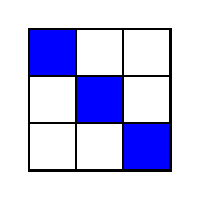
\begin{tikzpicture}
        [%%%%%%%%%%%%%%%%%%%%%%%%%%%%%%
        box/.style={rectangle,draw=black,thick, minimum size=0.6cm},
        ]%%%%%%%%%%%%%%%%%%%%%%%%%%%%%%
        
        \foreach \x in {0,1,...,2}{
          \foreach \y in {0,1,...,2}
          \node[box] at (\x*0.6,\y*0.6){};
        }
        
        \node[box,fill=blue ] at (0.6*0,0.6*2){};  
        \node[box,fill=blue ] at (0.6*1,0.6*1){};  
        \node[box,fill=blue ] at (0.6*2,0.6*0){};  
        
      \end{tikzpicture}
    \end{minipage}
    \begin{minipage}{0.3\textwidth}
      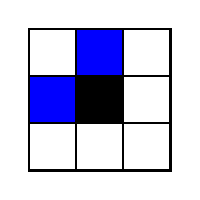
\begin{tikzpicture}
        [%%%%%%%%%%%%%%%%%%%%%%%%%%%%%%
        box/.style={rectangle,draw=black,thick, minimum size=0.6cm},
        ]%%%%%%%%%%%%%%%%%%%%%%%%%%%%%%
        
        \foreach \x in {0,1,...,2}{
          \foreach \y in {0,1,...,2}
          \node[box] at (\x*0.6,\y*0.6){};
        }
        
        \node[box,fill=black ] at (0.6*1,0.6*1){};  
        \node[box,fill=blue ] at (0.6*0,0.6*1){};  
        \node[box,fill=blue ] at (0.6*1,0.6*2){};  
        
      \end{tikzpicture}
    \end{minipage}
    \begin{minipage}{0.4\textwidth}
      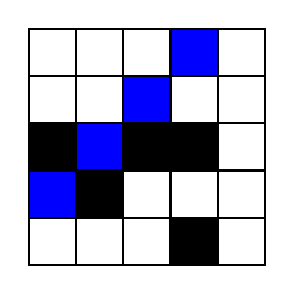
\begin{tikzpicture}
        [%%%%%%%%%%%%%%%%%%%%%%%%%%%%%%
        box/.style={rectangle,draw=black,thick, minimum size=0.6cm},
        ]%%%%%%%%%%%%%%%%%%%%%%%%%%%%%%
        
        \foreach \x in {0,1,...,4}{
          \foreach \y in {0,1,...,4}
          \node[box] at (\x*0.6,\y*0.6){};
        }
        
        \node[box,fill=black ] at (0.6*1,0.6*1){};  
        \node[box,fill=black ] at (0.6*0,0.6*2){};  
        \node[box,fill=black ] at (0.6*3,0.6*0){};  
        \node[box,fill=black ] at (0.6*3,0.6*2){};  
        \node[box,fill=black ] at (0.6*2,0.6*2){};  
        
        \node[box,fill=blue ] at (0.6*0,0.6*1){};  
        \node[box,fill=blue ] at (0.6*1,0.6*2){};  
        \node[box,fill=blue ] at (0.6*2,0.6*3){};  
        \node[box,fill=blue ] at (0.6*3,0.6*4){};  
      \end{tikzpicture}
      \end{minipage}
      
      Thus the expected answer for these three examples are 3, 2, and
      4 respectively.
      

\end{document}

%%% Local Variables:
%%% mode: latex
%%% TeX-master: t
%%% End:
